\documentclass[journal, a4paper]{IEEEtran}
\usepackage[italian]{babel}
\usepackage{booktabs}
\usepackage{siunitx}%Questo serve a caricare il pacchetto delle unità di misura del sistema internazionale%
\usepackage[utf8]{inputenc}
\usepackage{graphicx} 
\usepackage{url}
\usepackage{amsmath}
\usepackage{amssymb}


\usepackage{keyval}
\usepackage{xcolor}
\usepackage{caption}
\usepackage{subfig}
\usepackage{tikz}
\usepackage{circuitikz}
\usepackage{authblk}
%\usepackage{hyperref}

\begin{document}


% Define document title and author
	\title{Tecnologie Digitali - Logbook Week 15}
	\author[1]{Salvatore Bottaro}
		\author[2]{Lorenzo M. Perrone}
		\affil[1]{\texttt{salvo.bottaro@hotmail.it}}
		\affil[2]{\texttt{lorenzo.perrone.lmp@gmail.com}}
	\markboth{Tecnologie Digitali - Di Lieto}{}
	\maketitle
	
\begin{abstract}
	Logbook di laboratorio di Tecnologie Digitali, a.a. 2015/2016. Week 15
\end{abstract}

\section{Protocolli di comunicazione}
In aggiunta alla comunicazione seriale attraverso la connessione USB, Arduino presenta la possibilità di trasmettere e ricevere dati (sempre in modalità seriale) tramite le porte TX e RX, rispettivamente. Le specifiche di trasmissione possono sembrare controintuitive rispetto l'usuale assegnazione 0 $\rightarrow$ FALSE e 1 $\rightarrow$ TRUE: quando non vi è passaggio di dati si è in modalità \textit{idle}, che corrisponde al valore TRUE ed è dato da una tensione \textbf{negativa} generalmente compresa fra -3V e -15V. Per iniziare la comunicazione viene trasmesso un bit FALSE di \textit{start}, la cui tensione è \textbf{positiva} e compresa fra 3V e 15V. Quindi seguono gli otto bit della parola digitale, dal meno significativo al più significativo, conclusi da uno stato di \textit{stop}, TRUE, e quindi di nuovo in idle.\\
Se il baud viene settato a 9600, ci aspettiamo che fra l'inizio di due bit consecutivi ci sia appunto 1/9600 di secondo, pari circa a 0.104ms.\\
La sequenza riportata sulla scheda, 01001011, in codifica decimale corrisponde al numero 75, che a sua volta corrisponde al carattere ASCII \textbf{K}.\\

Consideriamo ora il seguente sketch di Arduino che realizza una comunicazione seriale con il computer e realizziamo gli opportuni collegamenti: la CB29 (GND) è collegata alla porta ADC0, TX è collegato sia alla CB68, che alla CB11, mentre invece la porta RX è scollegata. Con lo sketch caricato, viene trasmesso il carattere 'a', che corrisponde alla sequenza 00110001 (49 dec, 31 hex): tramite i cursori disponibili sul VI \textsc{TXRX} riusciamo a stimare l'intervallo fra un bit e l'altro, pari circa a 0.1ms, come ci aspettavamo.\\
Vediamo, tuttavia, che le specifiche di trasmissione dell'ATmega non corrispondono con quelle esposte precedentemente caratteristiche dello standard RS-232: l'ATmega, infatti, mantiene l'usuale 0 $\rightarrow$ FALSE e 1 $\rightarrow$ TRUE, dove il livello basso è a terra, e quello alto a 5V.\\

Come ulteriore prova, trasmettiamo il carattere ASCII 'X'. Ci aspettiamo una sequenza di stati (codificati secondo le specifiche ATmega) come in Figura (), e il risultato è invece in Figura (\ref{fig:es5_X}).\\

\begin{figure}
\centering
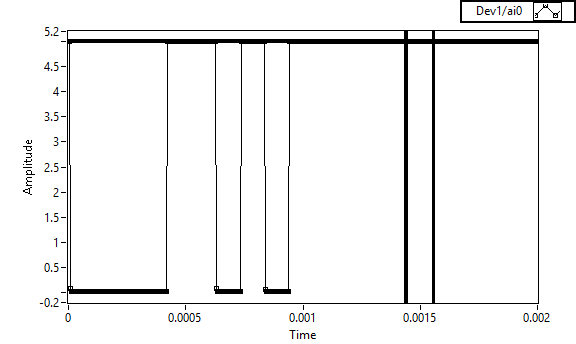
\includegraphics[width=0.9\linewidth]{./es5_X}
\caption{Carattere ASCII 'X'}
\label{fig:es5_X}
\end{figure}

Vediamo ora come si comporta la trasmissione di due caratteri consecutivi, senza ritardo fra di essi. I caratteri scelti sono '@' e '(', scelti in modo da facilitare il riconoscimento visivo, poichè il primo corrisponde alla sequenza 01000000, e il secondo a 00101000. Il risultato è in Figura (\ref{fig:es6_consecutive}). Come si osserva, i caratteri vengono trasmessi senza che vi siano pause fra il bit di stop del primo e il bit di start del secondo. 

\begin{figure}
\centering
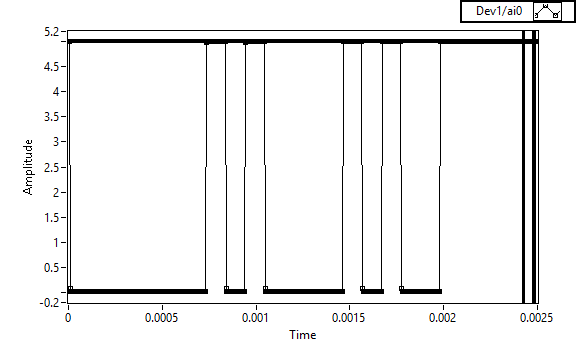
\includegraphics[width=0.9\linewidth]{./es6_consecutive}
\caption{Esercizio 6: due caratteri consecutivi}
\label{fig:es6_consecutive}
\end{figure}

Il comportamento che si verifica quando invece si introduce un delay fra la trasmissione dei due caratteri è più interessante: effettuando diverse prove si nota che il ritardo viene calcolato fra l'invio (e quindi l'inizio di trasmissione) dei caratteri, e non fra il bit di stop del primo e quello di start del secondo. Per questo motivo, se il ritardo è inferiore a 1ms (8+2 bit), questo non viene mostrato e i due dati vengono trasmessi consecutivamente, come nel caso precedente. Il motivo di questo comportamento è dovuto al fatto che l'ordine di trasmissione viene inviato dall'ATmega ad un componente esterno ad esso, che prevede l'eventualità che gli ordini vengano messi in coda, qualora questi dovessero sovrapporsi.

\begin{thebibliography}{5}

	%Each item starts with a \bibitem{reference} command and the details thereafter.
	
	\bibitem{JH6} % Conference paper
	Product data sheet: Dual Type D Flip-Flop \textsc{mc14013b}.
	\url{http://onsemi.com}

	\bibitem{M06} % Conference paper
	Paul Horowitz, Winfield Hill - The Art of Electronics. Cambridge University Press (1989).
	
\end{thebibliography}


\end{document}